\documentclass{thesis}
\usepackage[margin=0.5in]{geometry}
\documentclass[a4paper,10pt,draft]{thesis}
\usepackage{physics,amsmath, amsfonts, siunitx, amssymb, graphicx, slashed,subcaption}
\usepackage[utf8]{inputenc}
\usepackage[margin=1in]{geometry}
\usepackage[hidelinks]{hyperref}
\usepackage{xr-hyper}
\newcommand{\n}[1]{\nu_{#1}}
\newcommand{\na}{\nu_\alpha}
\newcommand{\nb}{\nu_\beta}
\newcommand{\ana}{\bar{\nu}_\alpha}
\newcommand{\an}[1]{\bar{\nu}_{\text{#1}}}
\newcommand{\anb}{\bar{\nu}_\beta}
\renewcommand{\a}{\alpha}
\renewcommand{\b}{\beta}
\newcommand{\ab}{\alpha\beta}


\renewcommand{\ne}{\nu_e}
\newcommand{\nm}{\nu_\mu}
\newcommand{\nt}{\nu_\tau}
\newcommand{\ns}{\nu_s}

\newcommand{\ane}{\bar{\nu}_e}
\newcommand{\anm}{\bar{\nu}_\mu}
\newcommand{\ant}{\bar{\nu}_\tau}
\newcommand{\ans}{\bar{\nu}_s}

\newcommand{\nee}{\nu_e \to \nu_e}
\newcommand{\nem}{\nu_e \to \nu_\mu}
\newcommand{\net}{\nu_e \to \nu_\tau}
\newcommand{\nes}{\nu_e \to \nu_s}

\newcommand{\nme}{\nu_\mu \to \nu_e}
\newcommand{\nmm}{\nu_\mu \to \nu_\mu}
\newcommand{\nmt}{\nu_\mu \to \nu_\tau}
\newcommand{\nms}{\nu_\mu \to \nu_s}



\newcommand{\Pee}{P_{e  e}}
\newcommand{\Pem}{P_{e  \mu}}
\newcommand{\Pet}{P_{e  \tau}}
\newcommand{\Pes}{P_{e  s}}

\newcommand{\Pme}{P_{\mu  e}}
\newcommand{\Pmm}{P_{\mu\mu}}
\newcommand{\Pmt}{P_{\mu  \tau}}
\newcommand{\Pms}{P_{\mu  s}}


\newcommand{\Pte}{P_{P_{\tau e}}}
\newcommand{\Ptm}{P_{\tau  \mu}}
\newcommand{\Ptt}{P_{\tau  \tau}}
\newcommand{\Pts}{P_{\mu  s}}

\newcommand{\Paeae}{P_{\bar{e}  \bar{e}}}
\newcommand{\Paeam}{P_{\bar{e}  \bar{\mu}}}
\newcommand{\Paeat}{P_{\bar{e}  \bar{\tau}}}
\newcommand{\Paeas}{P_{\bar{e}  \bar{s}}}

\newcommand{\Pamae}{P_{\bar{\mu}  \bar{e}}}
\newcommand{\Pamam}{P_{\bar{\mu}  \bar{\mu}}}
\newcommand{\Pamat}{P_{\bar{\mu}  \bar{\tau}}}
\newcommand{\Pamas}{P_{\bar{\mu}  \bar{s}}}


\newcommand{\Patae}{P_{\bar{\tau}  \bar{e}}}
\newcommand{\Patam}{P_{\bar{\tau}  \bar{\mu}}}
\newcommand{\Patat}{P_{\bar{\tau}  \bar{\tau}}}
\newcommand{\Patas}{P_{\bar{\mu}  \bar{s}}}

\renewcommand{\th}[1][]{%
  \theta\ifx\\#1\\\else_\text{#1}\fi
}
\newcommand{\thm}[1][]{%
  \theta^\text{M}\ifx\\#1\\\else_\text{#1}\fi
}
\renewcommand{\t}[1]{\text{{#1}}}
\newcommand{\avg}[1]{\left\langle {#1} \right \rangle}
\newcommand*{\dm}[1][]{%
  \Delta m^2\ifx\\#1\\\else_\text{#1}\fi
}
\newcommand{\zreco}{\cos{(\theta_z^{reco})}}
\newcommand{\ztrue}{\cos{(\theta_z^{true})}}
\newcommand{\z}{\cos{(\theta_z)}}
\newcommand{\Ereco}{E^{reco}}
\newcommand{\Etrue}{E^{true}}
\newcommand{\Aeff}{A^\text{eff}}
\newcommand{\emm}{\epsilon_{\mu\mu}}
\newcommand{\emt}{\epsilon_{\mu\tau}}
\newcommand{\eet}{\epsilon_{e\tau}}
\newcommand{\eem}{\epsilon_{e\mu}}
\newcommand{\ett}{\epsilon_{\tau\tau}}
\newcommand{\ep}{\epsilon^\prime}

\begin{document}
\begin{figure}[t]\label{fig:flux_aeff}
    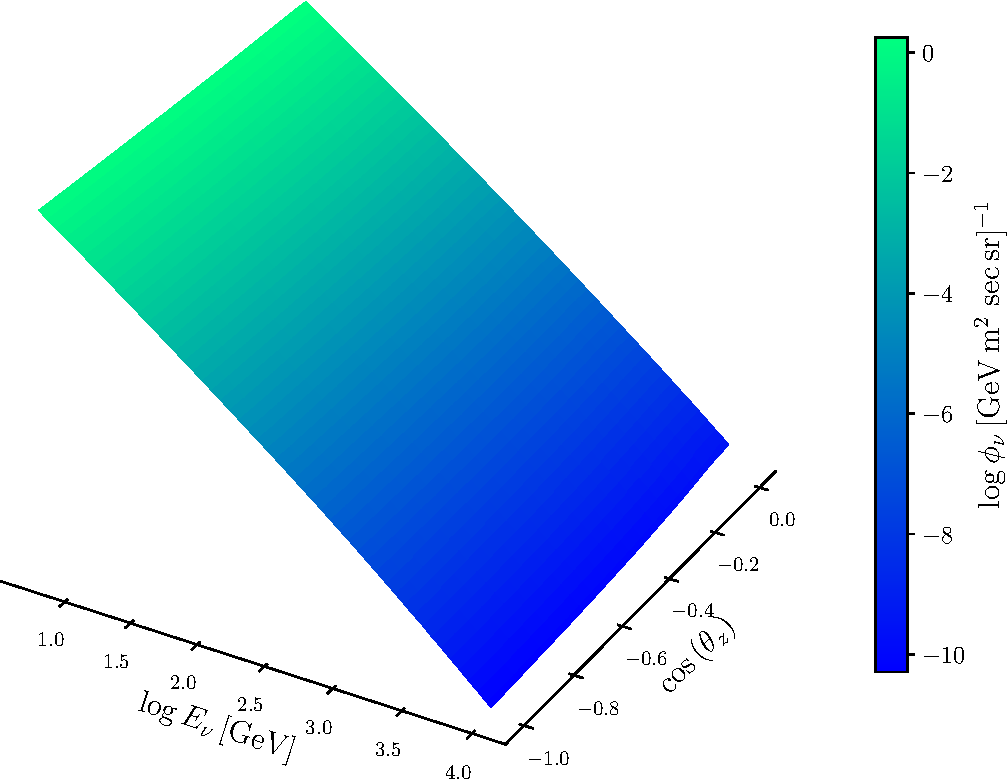
\includegraphics[width=0.5\textwidth]{figures/flux.pdf}\hspace{-1cm}
    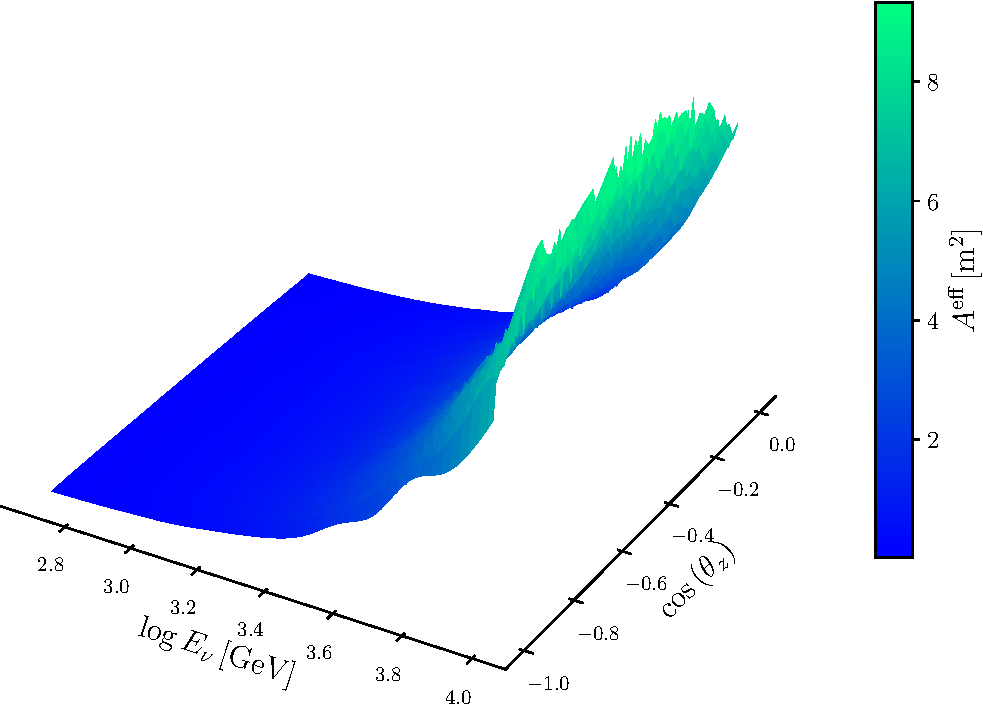
\includegraphics[width=0.5\textwidth]{figures/aeff.pdf}
    \vspace{-2.5cm}\caption{\emph{Left panel:} Interpolated South Pole atmospheric flux with data from~\cite{hondaArticle}.
    \emph{Right panel:} Interpolated IceCube effective area with data from~\cite{ICaeff}.}
\end{figure}

\section{Atmospheric neutrino flux}
Atmospheric neutrinos originates from cosmic rays composed of protons interacting with nuclei in the atmosphere.
These interactions ultimately produces pions, which decay as 
\begin{align}\label{eq:pion}
    \pi^+ &\to \mu^+ + \nm\,, \quad \pi^- \ to \mu^- + \anm \nonumber \\
    \pi^+ &\to e^+ + \ne\,, \quad \pi^- \ to e^- + \ane\,.
\end{align}
In the muonic decay channel, muons are emitted which will be detected by the IceCube detector. A part of the 
uncorrelated systematic error comes from this \emph{muon background}, i.e. events misclassified as muons from 
$\nm$ interactions rather than from pion decay. Moreover, the atmospheric flux is often associated with a large error.
In this work, we will use a flux normalization error of 24\%, and a zenith slope error of 4\%. In more sophisticated 
models, one can also include the pion to kaon flux uncertainty.

The flux is provided in \cite{hondaData,hondaArticle}, and a selection is shown in Table~\ref{table:flux}
The flux data is binned in $\ztrue$. The fluxes are averaged over azimuthal direction and over solar minimum/maximum. 
The units of the fluxes are given as \si{\per\GeV \per\metre\squared \per\second \per\steradian} and are omitted
from the table for clarity. 
We note that the fluxes for $\nt$ and $\nu_{\bar{\tau}}$ are missing. Kaons can decay into neutral pions, which in turn 
can produce $\nt$, but this branching ratio is extremely small. Thus, we never have to use probabilities on the form 
$P_{\tau \beta}$, since we have no incoming atmospheric $\nu_\tau$ flux. 

Interpolating the data yields makes us capable of returning all four necessary fluxes for a given true energy and true zenith.
The result is shown in Fig.~\ref{fig:flux_aeff}.

\begin{table}[h]\label{table:flux}
    \begin{center}
        \begin{tabular}{lcccccc}
            \hline \hline
            $\Etrue$ [\si{\GeV}] &$\phi_\mu$ &$\phi_{\bar{\mu}}$ &$\phi_e$ &$\phi_{\bar{e}}$ & $\ztrue_{min}$ &$\ztrue_{max}$\\
            \hline
            27825 &  \SI{6.06e-12}{} &  \SI{3.17e-12}{} &  \SI{1.56e-13}{} &  \SI{1.04e-13}{} &   -0.2 &   -0.1 \\
            247707 &  \SI{5.94e-16}{} &  \SI{2.92e-16}{} &  \SI{1.36e-17}{} &  \SI{8.12e-18}{} &   -0.7 &   -0.6 \\
                22 &  \SI{3.33e-02}{} &  \SI{2.78e-02}{} &  \SI{9.57e-03}{} & \SI{7.15e-03}{} &   -0.3 &   -0.2 \\
            432876 &  \SI{5.19e-17}{} &  \SI{2.32e-17}{} &  \SI{1.46e-18}{} & \SI{9.83e-19}{} &   -1.1 &   -1.0 \\
            64280 &  \SI{1.58e-13}{} &  \SI{8.10e-14}{} &  \SI{3.49e-15}{} &  \SI{2.21e-15}{} &   -0.4 &   -0.3 \\
            \hline
        \end{tabular}
    \end{center}
    \caption{A selection of processed atmospheric South Pole fluxes from~\cite{hondaData} by Honda et al.~\cite{hondaArticle}.}
\end{table}


\section{Event reconstruction}
After an event has occurred, the IceCube algorithms process the data coming from the detector to \emph{reconstruct} the event. This means that, given the parameters recorded by the detector, what are their "true" values?
We are interested in two variables: the energy and the direction. Each event is tagged with a probable energy and zenith angle, called the recostructed parameters $\Ereco$ and $\zreco$, which are the parameters according to the DOMs.
The collaboration then uses numerous sophisticated methods to backtrack the reconstructed parameters to the true parameters. So a charged lepton hits the DOMs, and we ultimately end up with the associated neutrino's true and reconstructed energy and zenith angle. The reconstructed parameters are what we are using to analyze the data (because this is what the detector actually sees), while the true parameters are used in the determination of that neutrino's "actual" flux and cross-section (because this is what nature sees).

How do we then translate between the reconstructed and true parameters? In this work, we are using two different methods, which are based on the form of data available to us. 

\section{IceCube event count}\label{ch:ICmethod}
As the neutrinos have propagated the Earth, they arrive at the South Pole, where they interact in the ice to form their charged leptons. We now are interested in the effective area, i.e.~the detector area that the lepton "sees".
The effective area, $\Aeff$, depends on several parameters, some of them being detector physical volume, $\Etrue$,$\ztrue$ and the neutrino cross-section. Fortunately, the binned $\Aeff$ is provided to us by the collaboration~\cite{ICaeff}.
The data file has the following form

\begin{table}\label{table:aeff}
    \begin{tabular}{lrrrrr}
        \hline \hline
        $\Etrue_{min}$ [\si{\GeV}] &     $\Etrue_{max}$ [\si{\GeV}]&   $\ztrue_{min}$ &   $\ztrue_{max}$ &     $\Aeff$ [\si{\metre\squared}] \\
        \hline
             251 &      316 &  -0.92 &  -0.91 &   0.0174 \\
          794300 &  1000000 &  -0.80 &  -0.79 &  69.3600 \\
            3981 &     5012 &  -0.78 &  -0.77 &   3.1490 \\
            1585 &     1995 &  -0.07 &  -0.06 &   0.4659 \\
            398 &      501 &  -0.73 &  -0.72 &   0.0555 \\
        \hline
        \end{tabular}
    \caption{IceCube effective area from~\cite{ICaeff}}
\end{table}

Here, $\Aeff$ has been averaged over $\Aeff_\mu$ and $\Aeff_{\bar{\mu}}$. Thus, it is not flavor dependent.
Just as with the fluxes, we interpolate this in $\Etrue,\ztrue$ and show the result %TODO aeff interpolation

So now we have the physical quantities in the true parameters. But as we discussed, we need a way to translate this into the reconstructed parameters that the detector gives us. We will call the relationship between 
$\Ereco$ and $\Etrue$ the energy resolution function, and the relationshop between $\zreco$ and $\ztrue$ the zenith resolution function. We assume the relationship to follow a logarithmic Gaussian distribution, giving it the form 
\begin{align}\label{eq:gaussian}
    R(x^r, x^t) = \frac{1}{\sqrt{2\pi} \sigma_{x^r}x^r} \exp\left[-\frac{(\log x^r-\mu(x^t))^2}{2\sigma_{x^r}^2}\right]\,.
\end{align}
The parameters of the Gaussian are $\sigma_{x^r}(x^t)$ and $\mu(x^t)$, which are functions of the true parameters. By multiplying the Gaussian in Eq.~\ref{eq:gaussian}, we are reweighing the values by the 
probability density of that point. This process is also called \emph{smearing} because it effectively spreads out the data around a certain point. 

So how do we then obtain $\sigma_{x^r}(x^t)$ and $\mu(x^t)$ needed to construct the Gaussian? A Monte Carlo sample publically released by the 
collaboration has all the ingredients that we need~\cite{IC2016}. In Table.~\ref{table:IC_MC} we show a selection of the data.
The "pdg" column refers to the Monte Carlo particle classification, where 13 is the tag for $\nm$, while -13 refers
to an $\anm$. Here we note a crucial property of the IceCube dataset that will impact our analysis: the MC released by the collaboration
only includes simulated muon events.

\begin{table}\label{table:IC_MC}
    \begin{tabular}{lrrrrr}
        \hline \hline
        pdg &      $\Ereco$ [\si{\GeV}] &     $\zreco$ &       $\Etrue$ [\si{\GeV}] &     $\ztrue$ \\
        \hline
         13 &  1665 & -0.645884 &    592 & -0.653421 \\
         13 &   587 & -0.373241 &    342 & -0.424979 \\
        -13 &  1431 & -0.177786 &   1169 & -0.189949 \\
        -13 &   831 & -0.807226 &   1071 & -0.805559 \\
         13 &   988 & -0.370746 &   1861 & -0.367922 \\
         \hline
  \end{tabular}
  \caption{A selection of the data found in~\ref{IC2016}}
\end{table}

First, we let $\zreco = \ztrue$ for all values. The angular resolution in IceCube for track-like events is less than $\SI{2}{\degree}$, making $\ztrue$ coincide with $\zreco$ for our study~\cite{IC2020}.
Thus, we only need to concern ourselves with the energy resolution.
In Fig.~\ref{fig:IC_MC_gpr}, we have plotted all event counts found in the MC file, over 8 million. However, this is too much data to process efficiently, with many outliers that ultimately don't weigh in 
that much in the final event count. To resolve this, we have opted to train a Gaussian process regressor on the dataset, from which we can extract the predicted mean and standard deviation for a point.
When doing this over $\Ereco$, we sample $\Etrue$ in the 99\%th percentile around the predicted mean. We then obtain the shaded band shown in Fig.~\ref{fig:IC_MC_gpr}. %TODO add plot with Etrue vs prob dens

The event rate for each bin reads
\begin{align}\label{eq:ICevents}
    N_{ij} &= T \int_{(\cos{\theta_z^r})_i}^{(\cos{\theta_z^r})_{i+1}} \dd \cos{\theta^r_z} \int_{E^r_{j}}^{E^r_{j+1}} \dd E^r \int_0^\pi R(\theta^r,\theta^t) \dd \cos{\theta^t} \int_0^\infty R(E^r,E^t) \dd E^t
    \times \left[ \sum_\beta \phi_\beta^\text{det}  A^\text{eff}_\beta\right]\,,
\end{align}
where $T$ is the live time of the detector.

\begin{figure}[!tb]\label{fig:IC_MC_gpr}
    \begin{center}
       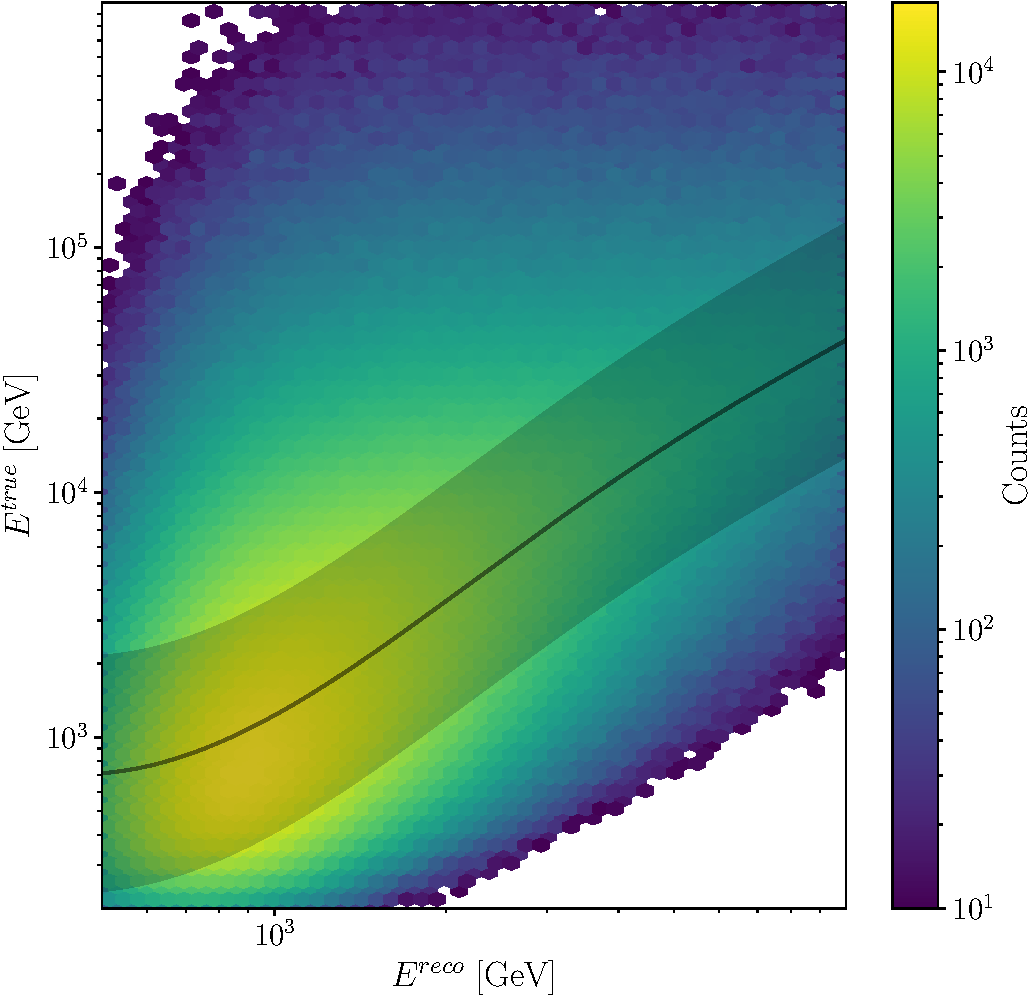
\includegraphics[width=0.4\linewidth]{figures/IC_MC_gpr.pdf}
    \end{center}
    \caption{Relationship between the true and reconstructed muon energy in the IceCube MC sample~\cite{IC2016}}\label{fig:IC_MC_counts}. Shaded area shows the $99.9$th percentile limits predicted by the regressor trained on this set.
 \end{figure}
\bibliographystyle{nature}
\bibliography{ref.bib}
\end{document}